\documentclass[11pt,a4paper]{article}
\usepackage[margin=2.2cm]{geometry}
\usepackage{booktabs}
\usepackage{graphicx}
\usepackage{amsmath}
\usepackage{float}
\usepackage[hidelinks]{hyperref}

\title{Assignment 6: Generative AI}
\author{}
\date{}

\begin{document}
\maketitle
\vspace{-1.5cm}

All models were trained on Fashion-MNIST (60k grayscale $28\times28$ images, 10 clothing classes).

\section{Part A: Denoising Autoencoder}

We trained two denoising autoencoders with a simple Conv-ReLU encoder/decoder architecture. The first reconstructs images corrupted with Gaussian noise ($\sigma=0.4$), the second removes a synthetic label overlay stamped on the image. Both were trained for 15 epochs with MSE loss.

\begin{figure}[H]
\centering
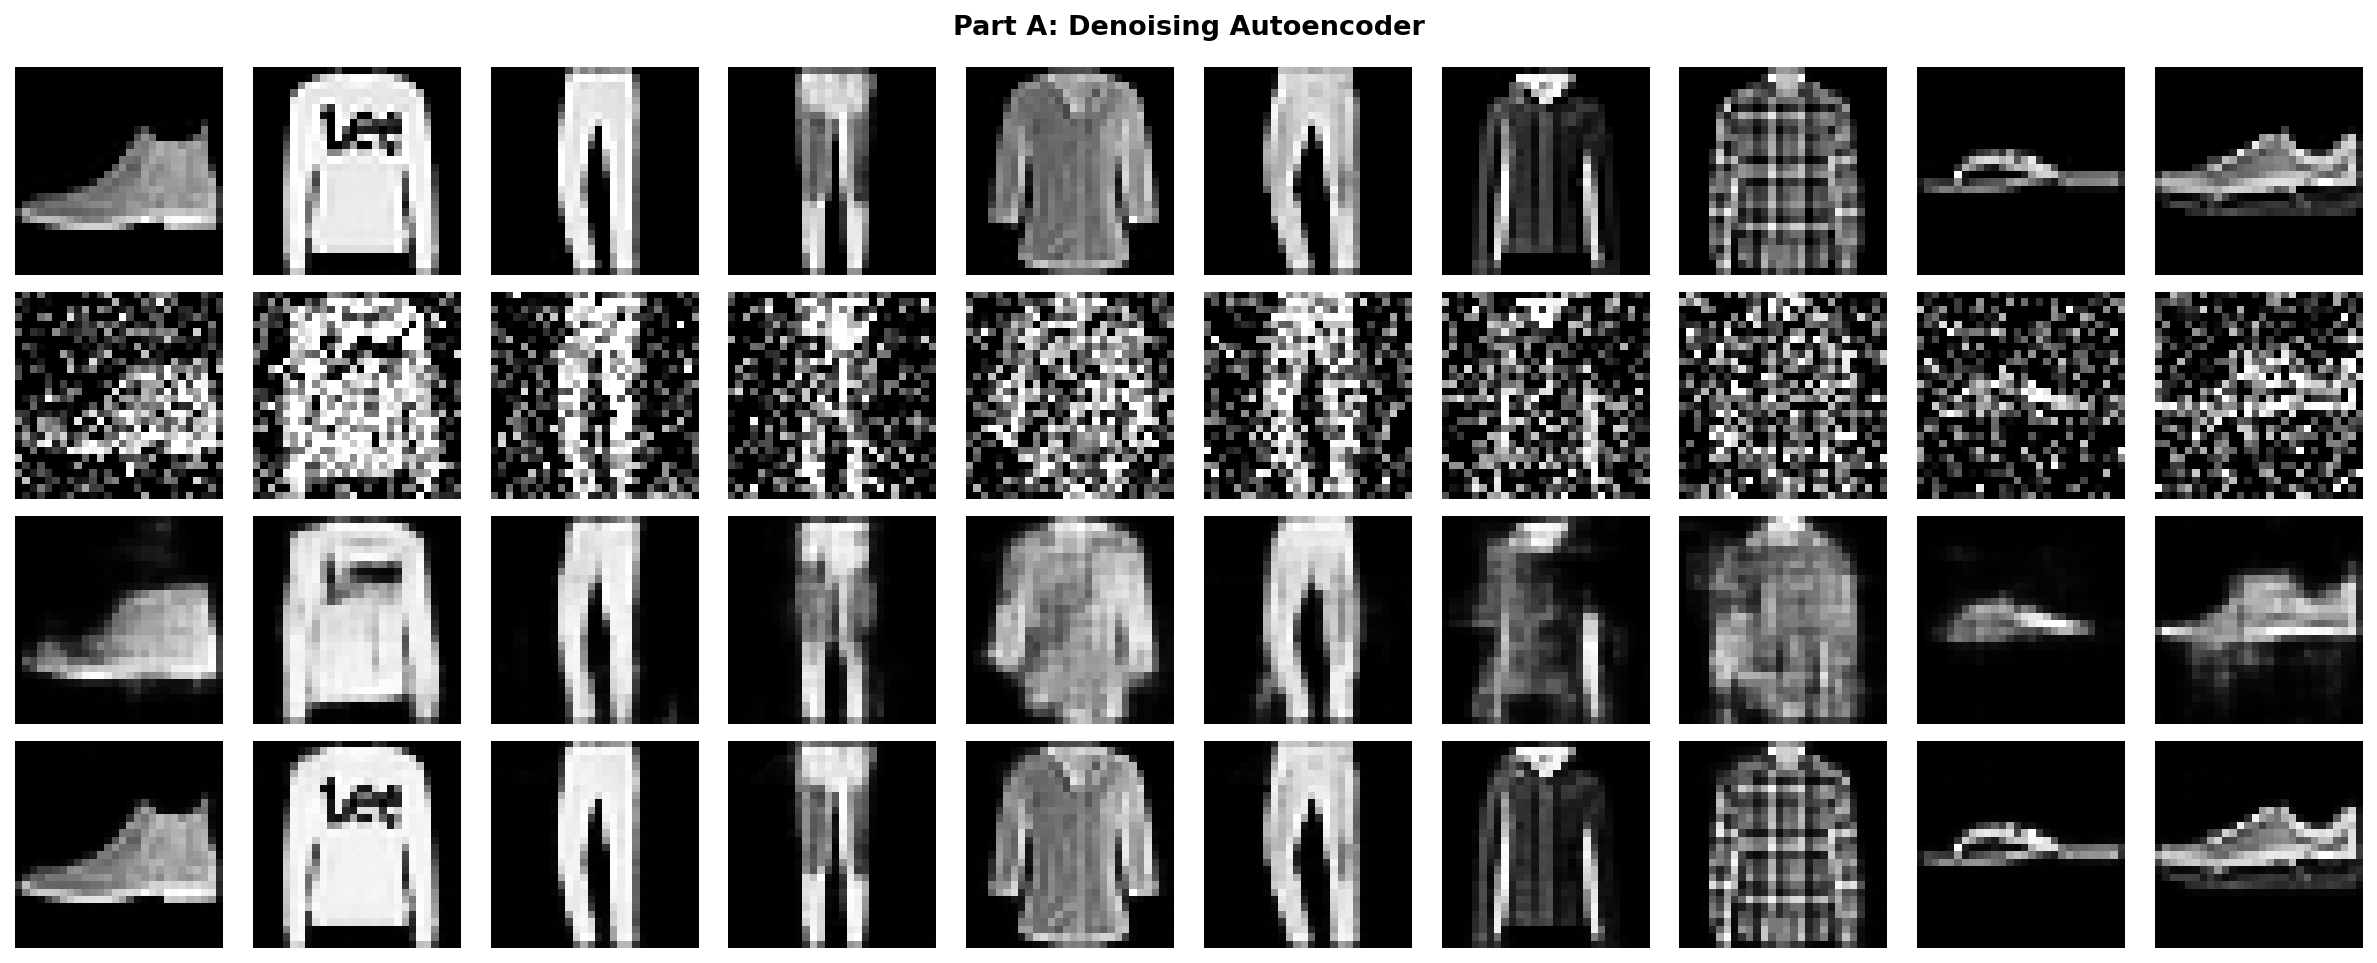
\includegraphics[width=0.95\textwidth]{part_a_denoising.png}
\caption{Row 1: originals, Row 2: Gaussian-noisy inputs, Row 3: denoised (Gaussian), Row 4: label-overlay denoised.}
\end{figure}

The Gaussian denoiser successfully recovers overall shape and contrast but produces slightly blurry outputs, as MSE loss averages over possible reconstructions. The label-overlay model learns to inpaint the corrupted region almost perfectly (loss dropped to 0.001), since the corruption is spatially localised and systematic. The denoising autoencoder does not generate novel images -- it only reconstructs corrupted inputs, making it a conditional generative model.

\section{Part B: Variational Autoencoder}

The VAE encoder outputs $\mu(x)$ and $\log\sigma^2(x)$ for a 32-dimensional latent space, with a symmetric convolutional decoder. Training uses the ELBO loss: binary cross-entropy reconstruction plus KL divergence $D_\mathrm{KL}(q(z|x) \| p(z))$. The loss converged from 291 to 240 over 20 epochs.

\begin{figure}[H]
\centering
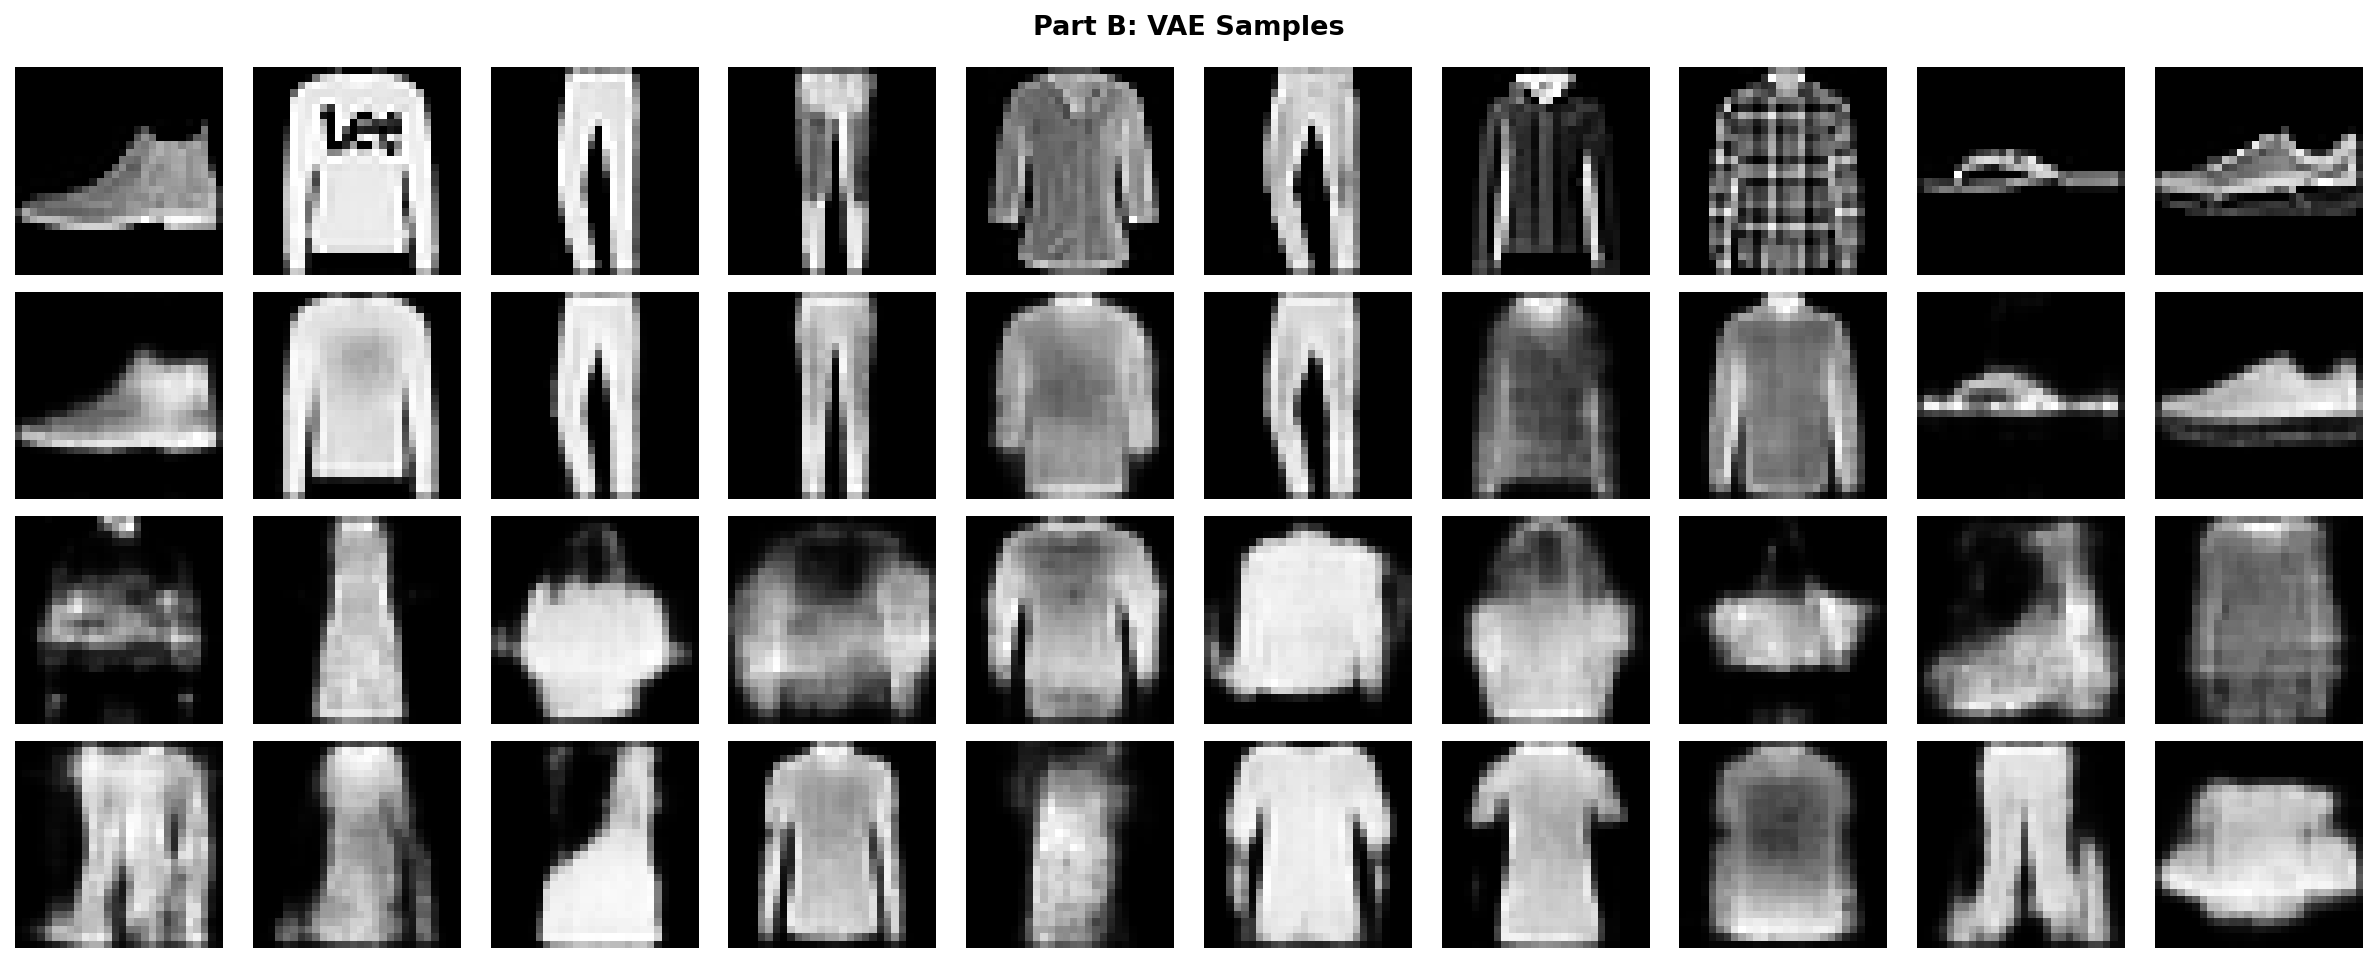
\includegraphics[width=0.95\textwidth]{part_b_vae.png}
\caption{Rows 1--2: original and reconstructed test images. Rows 3--4: random samples from $z \sim \mathcal{N}(0, I)$.}
\end{figure}

VAE reconstructions preserve global structure but are blurry, a well-known consequence of the pixel-wise reconstruction loss which penalises sharpness. Generated samples from random latent vectors produce recognisable clothing items (shirts, trousers, shoes) with coherent silhouettes, confirming the latent space is smooth and structured. The KL term ensures the latent distribution stays close to $\mathcal{N}(0, I)$, which enables meaningful random sampling but trades off reconstruction fidelity.

\section{Part C: GAN}

We trained a DCGAN-style generator $G(z) \to \hat{x}$ and discriminator $D(x) \to [0,1]$ with a 64-d latent space for 30 epochs. The discriminator loss stabilised near 0.51, indicating approximate Nash equilibrium where $D$ assigns roughly 50\% probability to both real and fake images.

\begin{figure}[H]
\centering
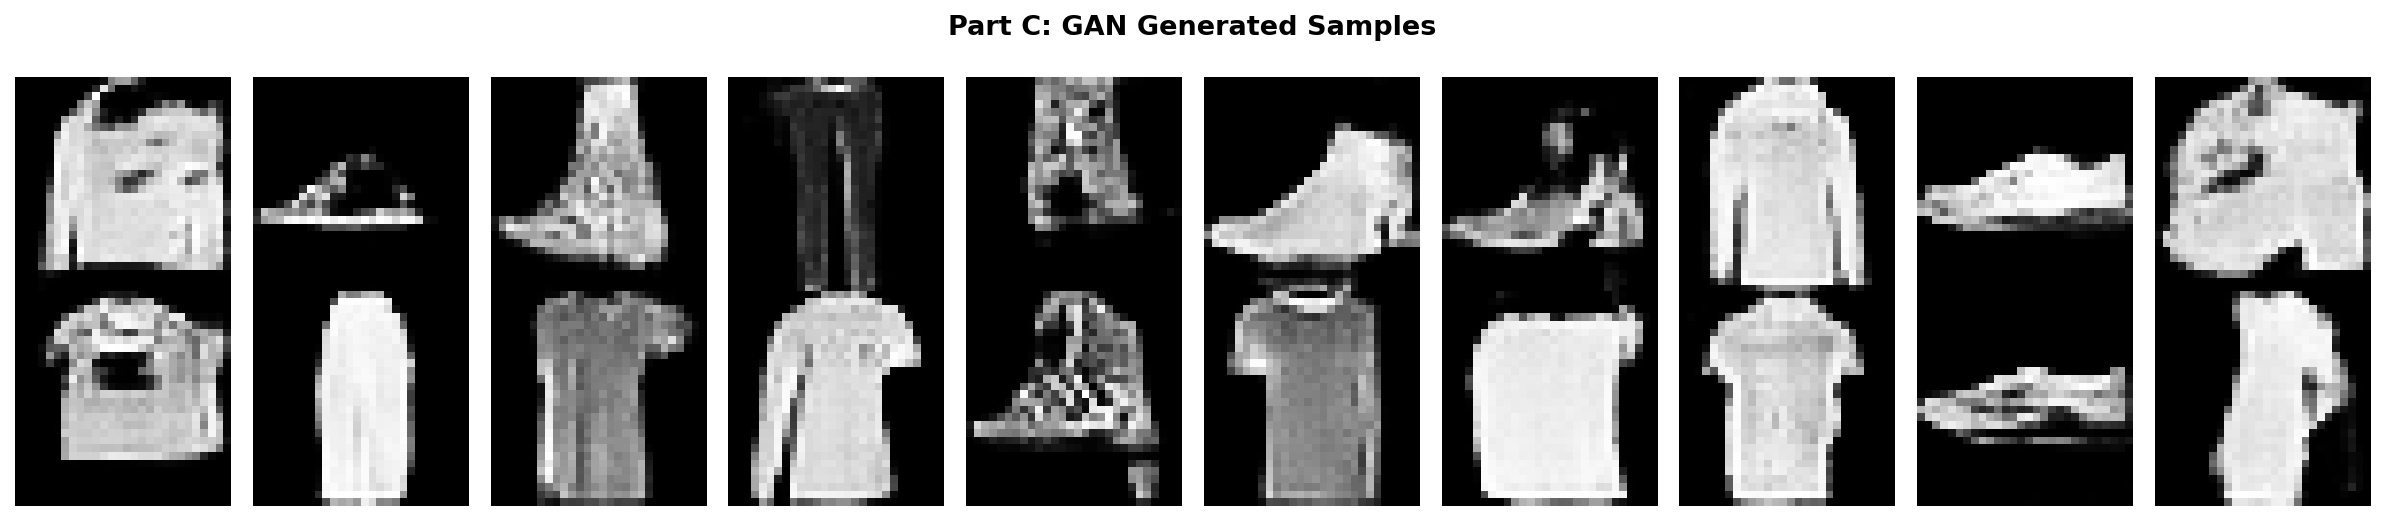
\includegraphics[width=0.95\textwidth]{part_c_gan.png}
\caption{GAN-generated samples from random noise vectors.}
\end{figure}

GAN samples are noticeably sharper than VAE outputs because the adversarial loss directly penalises unrealistic-looking images rather than pixel-level differences. The generated images show recognisable clothing items with clearer edges and more realistic textures. However, the GAN exhibits less diversity than the VAE -- several samples share similar poses and orientations, hinting at partial mode collapse where the generator focuses on a subset of the data distribution.

\section{Part D: Diffusion Model}

We implemented a DDPM with $T=300$ timesteps and a linear noise schedule ($\beta_1=10^{-4}$ to $\beta_T=0.02$). The denoising network is a small U-Net with sinusoidal timestep embeddings, trained for 20 epochs to predict the noise $\varepsilon$ added at each timestep.

\begin{figure}[H]
\centering
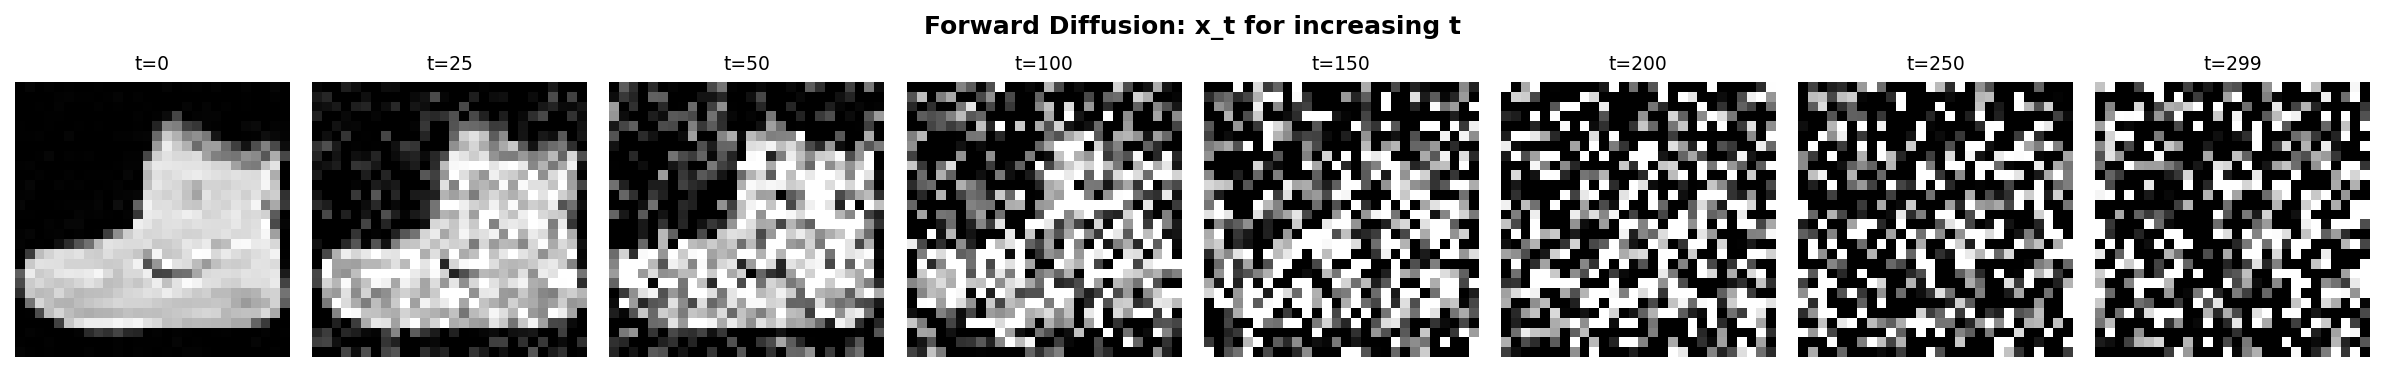
\includegraphics[width=0.95\textwidth]{part_d_forward_diffusion.png}
\caption{Forward diffusion: the image gradually becomes pure noise as $t$ increases.}
\end{figure}

\begin{figure}[H]
\centering
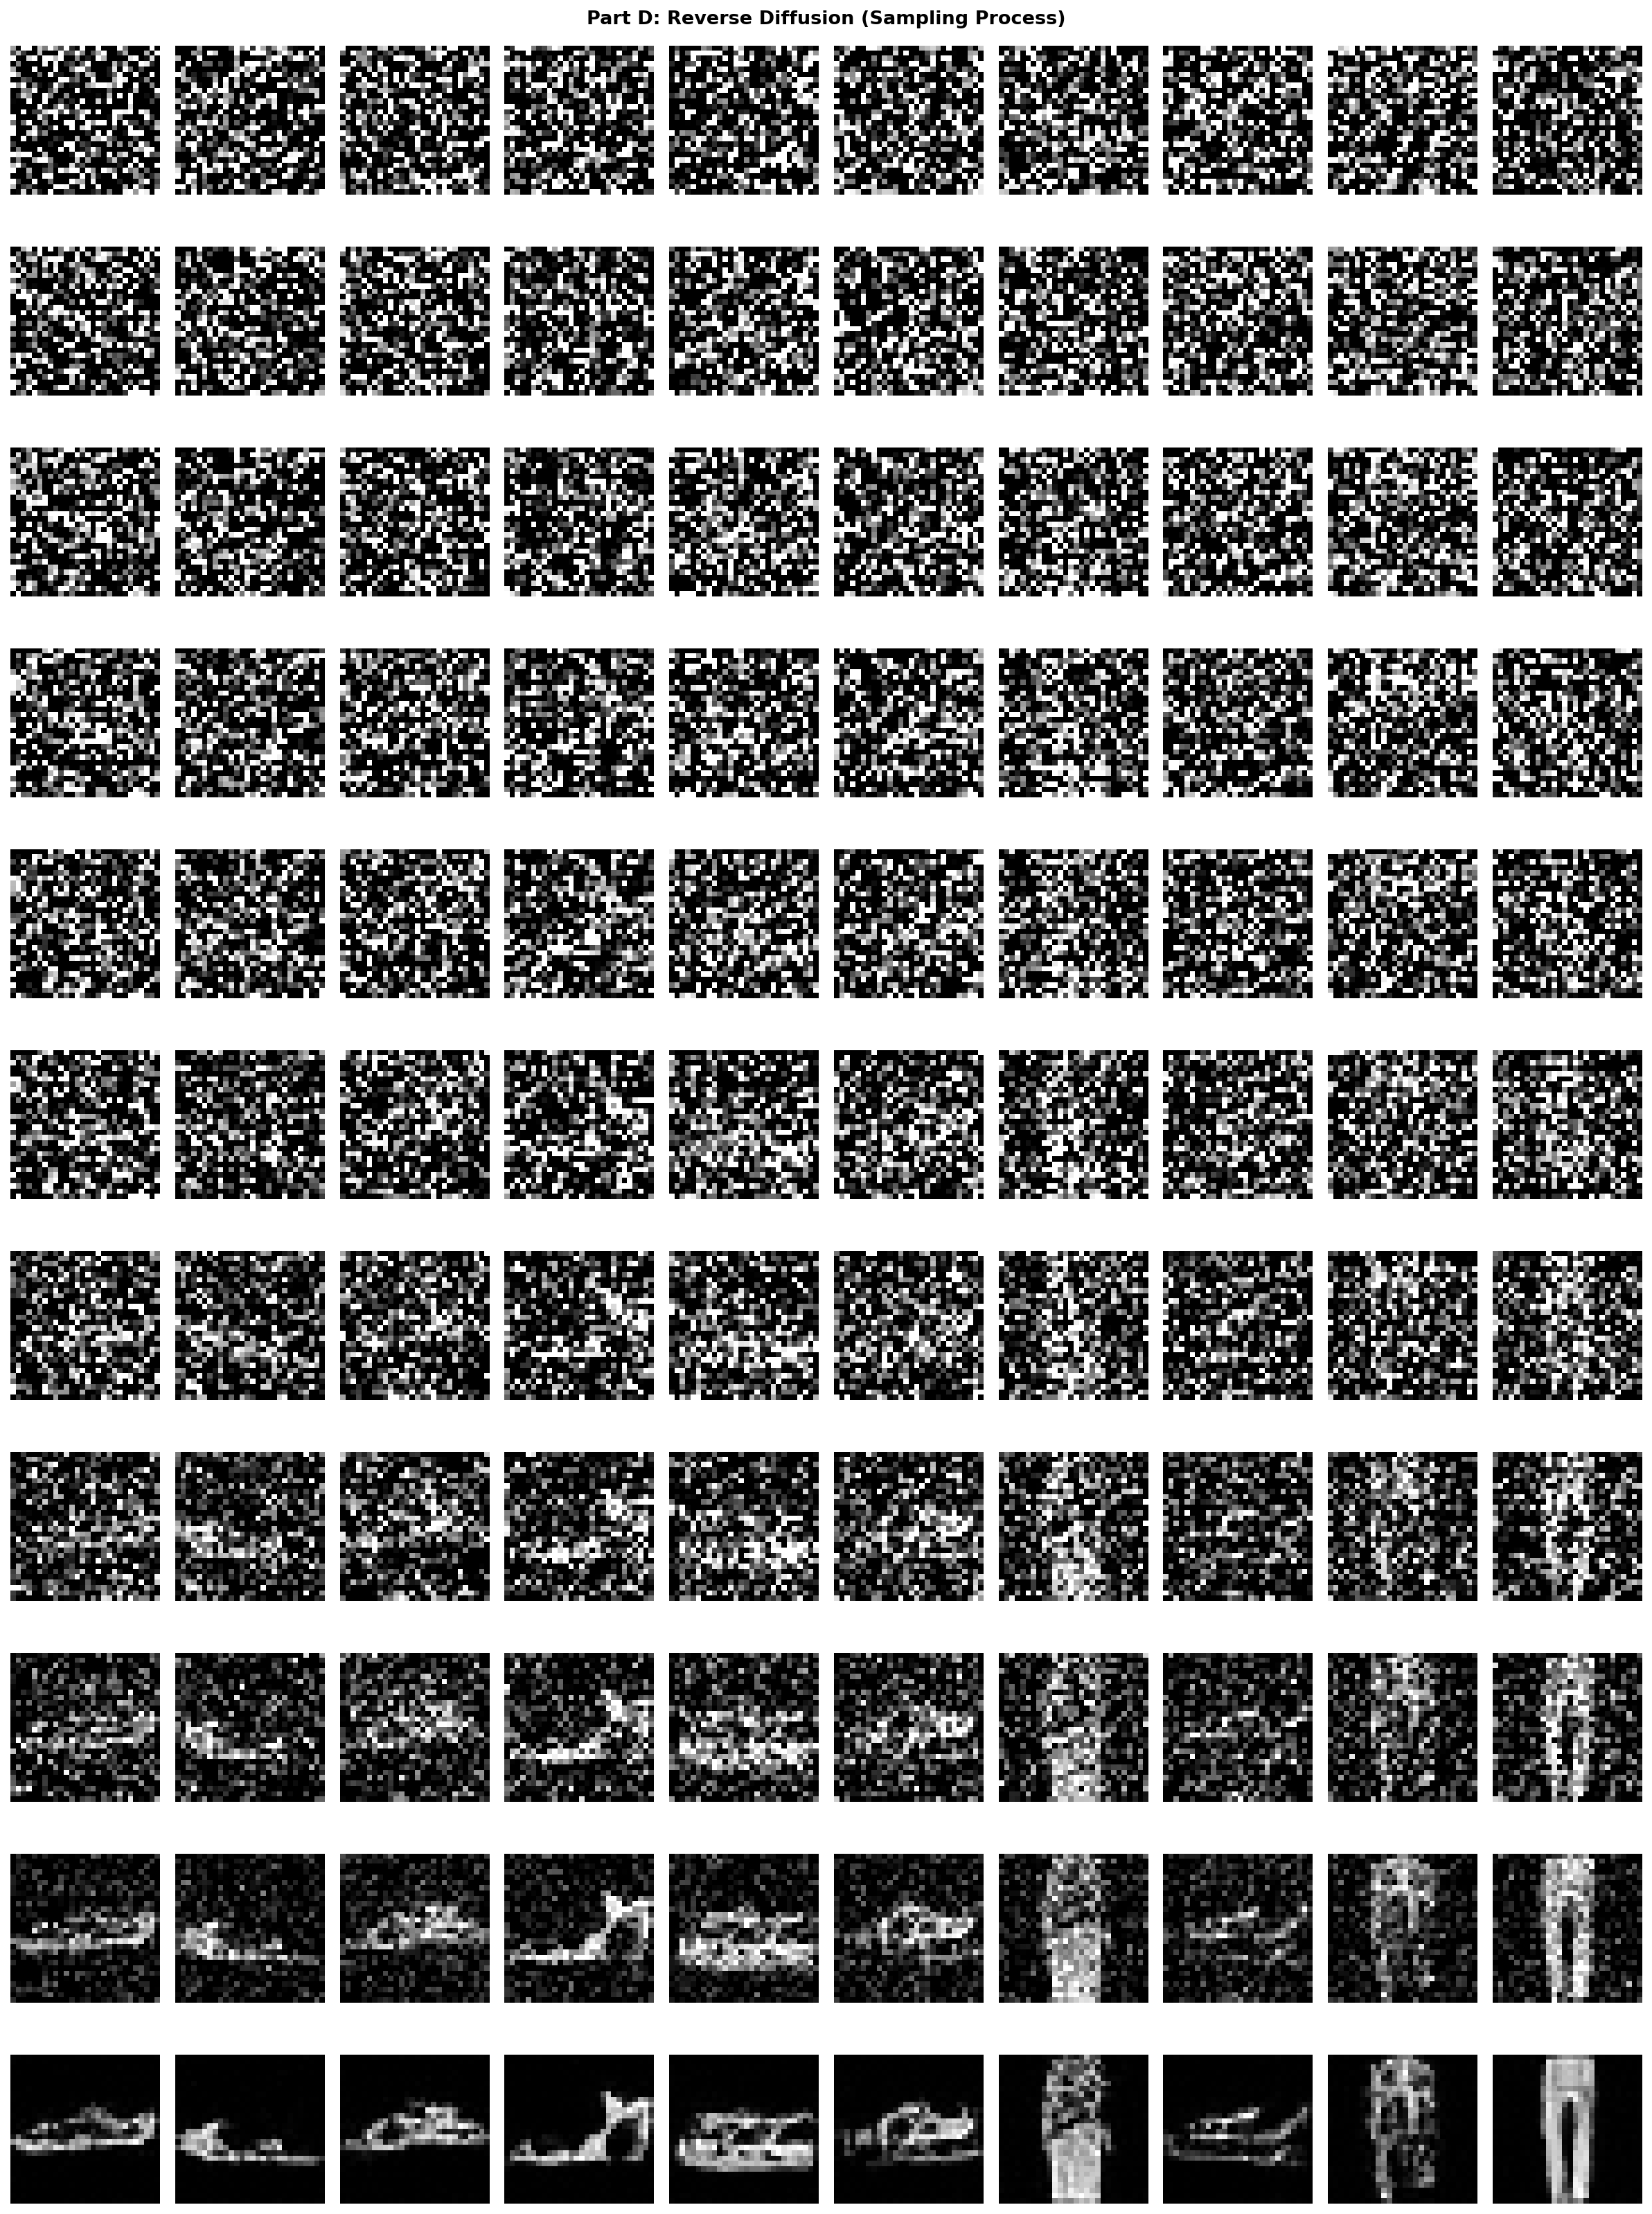
\includegraphics[width=0.65\textwidth]{part_d_sampling_process.png}
\caption{Reverse diffusion sampling: from noise ($t=300$) to generated image ($t=0$).}
\end{figure}

The forward process shows a smooth transition from clean image to Gaussian noise. Reverse sampling demonstrates the iterative denoising: structure emerges around $t=60$ and refines into recognisable shapes by $t=0$. With only 20 training epochs the generated samples are rough but show recognisable shoe and clothing shapes, confirming the model has learned meaningful denoising.

\section{Comparison}

\begin{figure}[H]
\centering
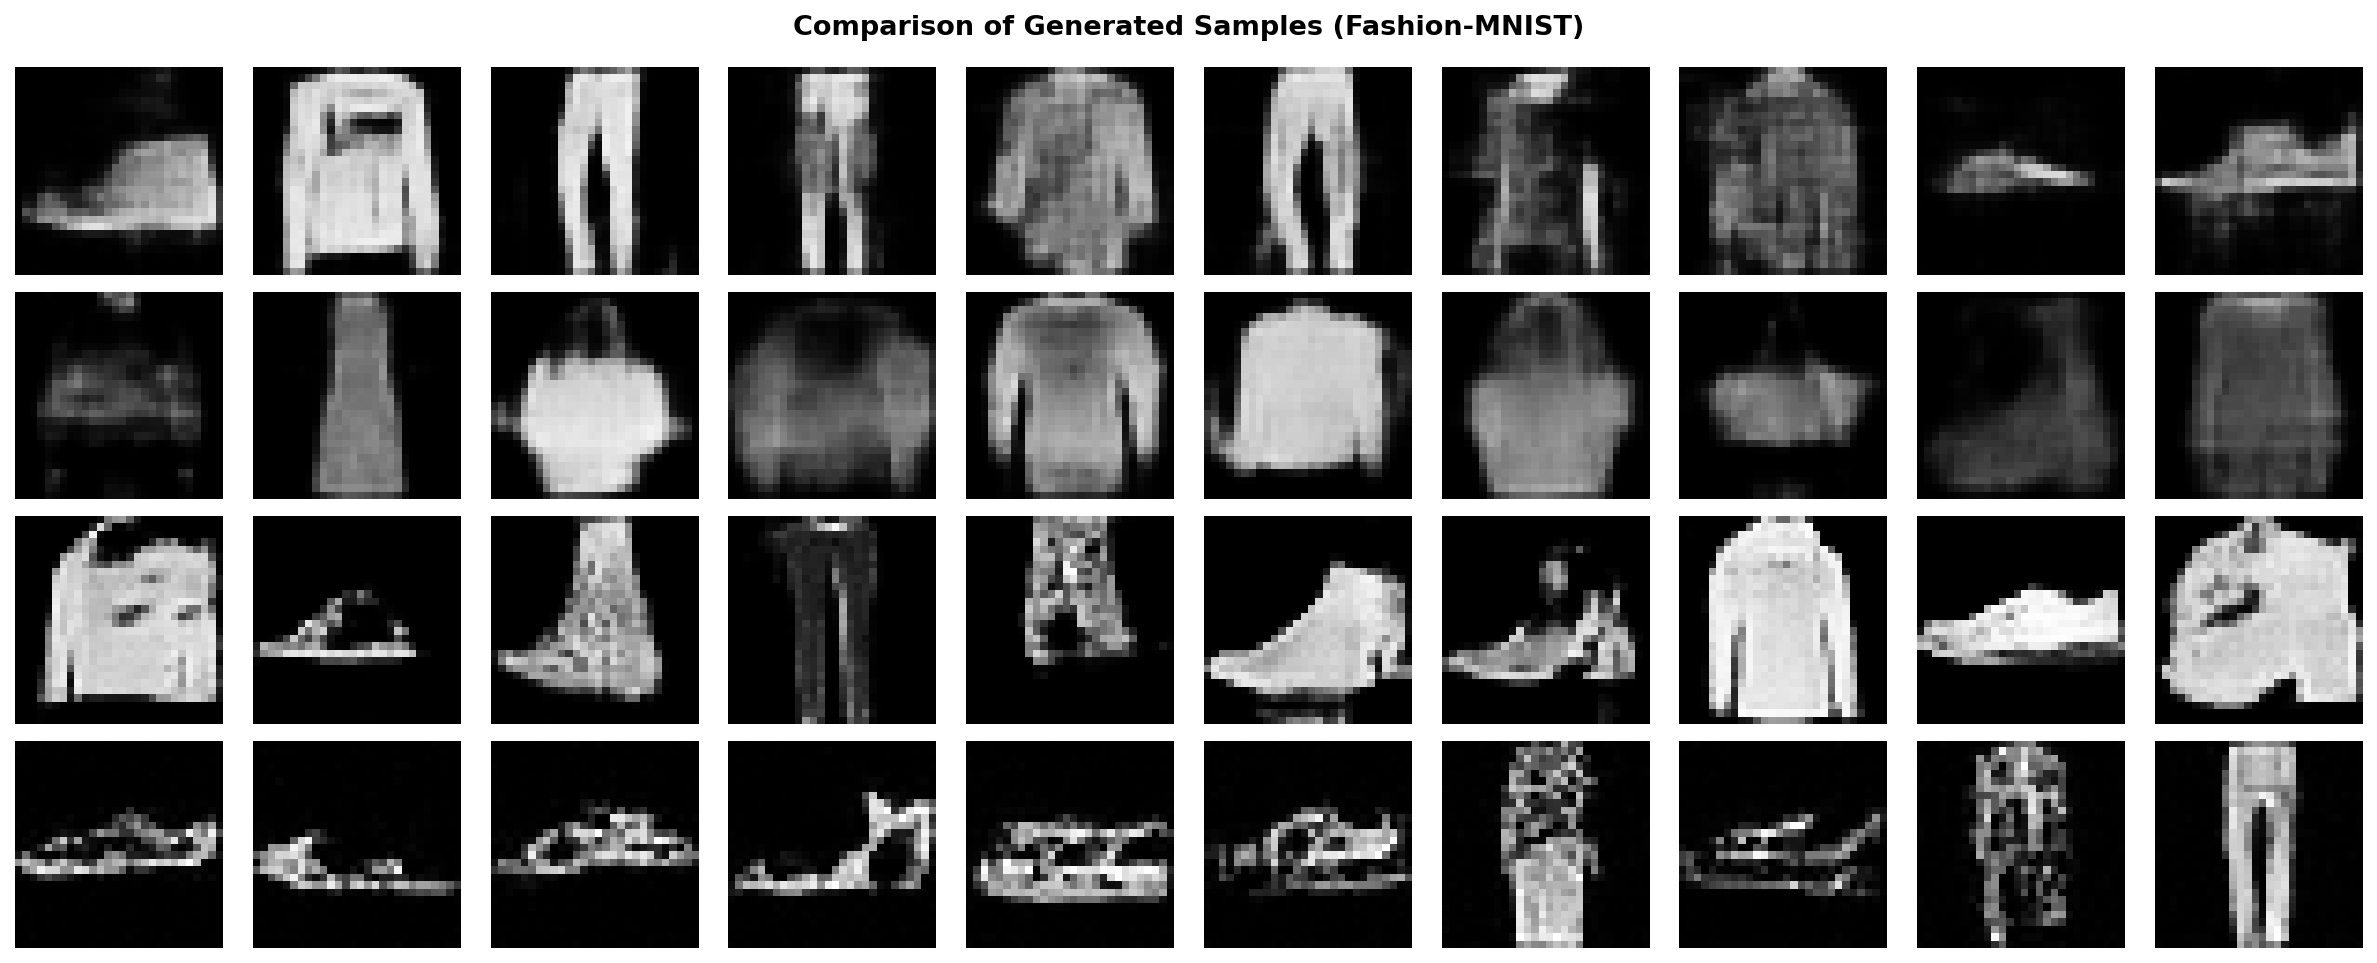
\includegraphics[width=0.95\textwidth]{comparison_all_models.png}
\caption{Side-by-side comparison of generated samples from all four models.}
\end{figure}

\begin{table}[H]
\centering
\begin{tabular}{lcccc}
\toprule
Property & DAE & VAE & GAN & Diffusion \\
\midrule
Sharpness & Medium & Low & High & Low \\
Diversity & N/A & High & Medium & Medium \\
Training stability & Stable & Stable & Fragile & Stable \\
Novel generation & No & Yes & Yes & Yes \\
\bottomrule
\end{tabular}
\caption{Qualitative comparison of generative model properties.}
\end{table}

The DAE produces the sharpest outputs but cannot generate novel images -- it only denoises existing ones. The VAE generates diverse samples but they are blurry due to the pixel-wise reconstruction loss. The GAN produces the sharpest novel samples thanks to adversarial training but risks mode collapse and is the hardest to train stably. The diffusion model produces reasonable samples with stable training but requires many more epochs and larger networks to match GAN quality. With sufficient compute, diffusion models typically surpass GANs in both quality and diversity, which explains their dominance in modern image generation systems.

\end{document}
